% Options for packages loaded elsewhere
\PassOptionsToPackage{unicode}{hyperref}
\PassOptionsToPackage{hyphens}{url}
%
\documentclass[
]{book}
\usepackage{lmodern}
\usepackage{amssymb,amsmath}
\usepackage{ifxetex,ifluatex}
\ifnum 0\ifxetex 1\fi\ifluatex 1\fi=0 % if pdftex
  \usepackage[T1]{fontenc}
  \usepackage[utf8]{inputenc}
  \usepackage{textcomp} % provide euro and other symbols
\else % if luatex or xetex
  \usepackage{unicode-math}
  \defaultfontfeatures{Scale=MatchLowercase}
  \defaultfontfeatures[\rmfamily]{Ligatures=TeX,Scale=1}
\fi
% Use upquote if available, for straight quotes in verbatim environments
\IfFileExists{upquote.sty}{\usepackage{upquote}}{}
\IfFileExists{microtype.sty}{% use microtype if available
  \usepackage[]{microtype}
  \UseMicrotypeSet[protrusion]{basicmath} % disable protrusion for tt fonts
}{}
\makeatletter
\@ifundefined{KOMAClassName}{% if non-KOMA class
  \IfFileExists{parskip.sty}{%
    \usepackage{parskip}
  }{% else
    \setlength{\parindent}{0pt}
    \setlength{\parskip}{6pt plus 2pt minus 1pt}}
}{% if KOMA class
  \KOMAoptions{parskip=half}}
\makeatother
\usepackage{xcolor}
\IfFileExists{xurl.sty}{\usepackage{xurl}}{} % add URL line breaks if available
\IfFileExists{bookmark.sty}{\usepackage{bookmark}}{\usepackage{hyperref}}
\hypersetup{
  pdftitle={Statistik (B.Sc. Data Science)},
  pdfauthor={Prof.~Dr.~Dominik Liebl},
  hidelinks,
  pdfcreator={LaTeX via pandoc}}
\urlstyle{same} % disable monospaced font for URLs
\usepackage{color}
\usepackage{fancyvrb}
\newcommand{\VerbBar}{|}
\newcommand{\VERB}{\Verb[commandchars=\\\{\}]}
\DefineVerbatimEnvironment{Highlighting}{Verbatim}{commandchars=\\\{\}}
% Add ',fontsize=\small' for more characters per line
\usepackage{framed}
\definecolor{shadecolor}{RGB}{248,248,248}
\newenvironment{Shaded}{\begin{snugshade}}{\end{snugshade}}
\newcommand{\AlertTok}[1]{\textcolor[rgb]{0.94,0.16,0.16}{#1}}
\newcommand{\AnnotationTok}[1]{\textcolor[rgb]{0.56,0.35,0.01}{\textbf{\textit{#1}}}}
\newcommand{\AttributeTok}[1]{\textcolor[rgb]{0.77,0.63,0.00}{#1}}
\newcommand{\BaseNTok}[1]{\textcolor[rgb]{0.00,0.00,0.81}{#1}}
\newcommand{\BuiltInTok}[1]{#1}
\newcommand{\CharTok}[1]{\textcolor[rgb]{0.31,0.60,0.02}{#1}}
\newcommand{\CommentTok}[1]{\textcolor[rgb]{0.56,0.35,0.01}{\textit{#1}}}
\newcommand{\CommentVarTok}[1]{\textcolor[rgb]{0.56,0.35,0.01}{\textbf{\textit{#1}}}}
\newcommand{\ConstantTok}[1]{\textcolor[rgb]{0.00,0.00,0.00}{#1}}
\newcommand{\ControlFlowTok}[1]{\textcolor[rgb]{0.13,0.29,0.53}{\textbf{#1}}}
\newcommand{\DataTypeTok}[1]{\textcolor[rgb]{0.13,0.29,0.53}{#1}}
\newcommand{\DecValTok}[1]{\textcolor[rgb]{0.00,0.00,0.81}{#1}}
\newcommand{\DocumentationTok}[1]{\textcolor[rgb]{0.56,0.35,0.01}{\textbf{\textit{#1}}}}
\newcommand{\ErrorTok}[1]{\textcolor[rgb]{0.64,0.00,0.00}{\textbf{#1}}}
\newcommand{\ExtensionTok}[1]{#1}
\newcommand{\FloatTok}[1]{\textcolor[rgb]{0.00,0.00,0.81}{#1}}
\newcommand{\FunctionTok}[1]{\textcolor[rgb]{0.00,0.00,0.00}{#1}}
\newcommand{\ImportTok}[1]{#1}
\newcommand{\InformationTok}[1]{\textcolor[rgb]{0.56,0.35,0.01}{\textbf{\textit{#1}}}}
\newcommand{\KeywordTok}[1]{\textcolor[rgb]{0.13,0.29,0.53}{\textbf{#1}}}
\newcommand{\NormalTok}[1]{#1}
\newcommand{\OperatorTok}[1]{\textcolor[rgb]{0.81,0.36,0.00}{\textbf{#1}}}
\newcommand{\OtherTok}[1]{\textcolor[rgb]{0.56,0.35,0.01}{#1}}
\newcommand{\PreprocessorTok}[1]{\textcolor[rgb]{0.56,0.35,0.01}{\textit{#1}}}
\newcommand{\RegionMarkerTok}[1]{#1}
\newcommand{\SpecialCharTok}[1]{\textcolor[rgb]{0.00,0.00,0.00}{#1}}
\newcommand{\SpecialStringTok}[1]{\textcolor[rgb]{0.31,0.60,0.02}{#1}}
\newcommand{\StringTok}[1]{\textcolor[rgb]{0.31,0.60,0.02}{#1}}
\newcommand{\VariableTok}[1]{\textcolor[rgb]{0.00,0.00,0.00}{#1}}
\newcommand{\VerbatimStringTok}[1]{\textcolor[rgb]{0.31,0.60,0.02}{#1}}
\newcommand{\WarningTok}[1]{\textcolor[rgb]{0.56,0.35,0.01}{\textbf{\textit{#1}}}}
\usepackage{longtable,booktabs}
% Correct order of tables after \paragraph or \subparagraph
\usepackage{etoolbox}
\makeatletter
\patchcmd\longtable{\par}{\if@noskipsec\mbox{}\fi\par}{}{}
\makeatother
% Allow footnotes in longtable head/foot
\IfFileExists{footnotehyper.sty}{\usepackage{footnotehyper}}{\usepackage{footnote}}
\makesavenoteenv{longtable}
\usepackage{graphicx,grffile}
\makeatletter
\def\maxwidth{\ifdim\Gin@nat@width>\linewidth\linewidth\else\Gin@nat@width\fi}
\def\maxheight{\ifdim\Gin@nat@height>\textheight\textheight\else\Gin@nat@height\fi}
\makeatother
% Scale images if necessary, so that they will not overflow the page
% margins by default, and it is still possible to overwrite the defaults
% using explicit options in \includegraphics[width, height, ...]{}
\setkeys{Gin}{width=\maxwidth,height=\maxheight,keepaspectratio}
% Set default figure placement to htbp
\makeatletter
\def\fps@figure{htbp}
\makeatother
\setlength{\emergencystretch}{3em} % prevent overfull lines
\providecommand{\tightlist}{%
  \setlength{\itemsep}{0pt}\setlength{\parskip}{0pt}}
\setcounter{secnumdepth}{5}
\usepackage{amsthm}
\usepackage{float}
\usepackage{rotating, graphicx}
\usepackage{multirow}
\usepackage{tabularx}

% new command for pretty oversets with \sim
\newcommand\simcal[1]{\stackrel{\sim}{\smash{\mathcal{#1}}\rule{0pt}{0.5ex}}}

\newcommand{\comma}{,\,}

\floatplacement{figure}{H}

\PassOptionsToPackage{table}{xcolor}

\usepackage{tcolorbox}

\definecolor{kcblue}{HTML}{D7DDEF}
\definecolor{kcdarkblue}{HTML}{2B4E70}

\makeatletter
\def\thm@space@setup{%
  \thm@preskip=8pt plus 2pt minus 4pt
  \thm@postskip=\thm@preskip
}
\makeatother

% \makeatletter % undo the wrong changes made by mathspec
% \let\RequirePackage\original@RequirePackage
% \let\usepackage\RequirePackage
% \makeatother

\newenvironment{rmdknit}
    {\begin{center}
    \begin{tabular}{|p{0.9\textwidth}|}
    \hline\\
    }
    {
    \\\\\hline
    \end{tabular}
    \end{center}
    }

\newenvironment{rmdnote}
    {\begin{center}
    \begin{tabular}{|p{0.9\textwidth}|}
    \hline\\
    }
    {
    \\\\\hline
    \end{tabular}
    \end{center}
    }

\newtcolorbox[auto counter, number within=section]{keyconcepts}[2][]{%
colback=kcblue,colframe=kcdarkblue,fonttitle=\bfseries, title=Key Concept~#2, after title={\newline #1}, beforeafter skip=15pt}
\usepackage[]{natbib}
\bibliographystyle{apalike}

\title{Statistik (B.Sc. Data Science)}
\author{Prof.~Dr.~Dominik Liebl}
\date{}

\begin{document}
\maketitle

{
\setcounter{tocdepth}{1}
\tableofcontents
}
\hypertarget{informationen}{%
\chapter*{Informationen}\label{informationen}}
\addcontentsline{toc}{chapter}{Informationen}

Dies ist das Skript zur Vorlesung \emph{Grundlagen der Statistik} (B.Sc. Data Science)

\hypertarget{vorlesungszeiten}{%
\subsection*{Vorlesungszeiten}\label{vorlesungszeiten}}
\addcontentsline{toc}{subsection}{Vorlesungszeiten}

\begin{table}[H]
\centering
\begin{tabular}[t]{l|l|l}
\hline
Wochentag & Uhrzeit & Ort (bzw. Zoom-Link)\\
\hline
Dienstag & 9:15-10:45 & Hörsaal 12.3\\
\hline
Freitag & 8:30-10:00 & Hörsaal 12.3\\
\hline
\end{tabular}
\end{table}

\hypertarget{leseecke}{%
\subsection*{Leseecke}\label{leseecke}}
\addcontentsline{toc}{subsection}{Leseecke}

Folgende \emph{frei zugängliche} Lehrbücher enthalten Teile dieses Kurses. In den jeweiligen Kapiteln, werde ich auf die einzelnen Bücher verweisen.

\begin{itemize}
\item
  \href{https://www.microsoft.com/en-us/research/uploads/prod/2006/01/Bishop-Pattern-Recognition-and-Machine-Learning-2006.pdf}{Pattern Recognition and Machine Learning} (by Christopher Bishop)
\item
  \href{https://trevorhastie.github.io/ISLR/}{An Introduction to Statistical Learning, with Applications in R} (by Gareth James, Daniela Witten, Trevor Hastie and Robert Tibshirani).
\item
  \href{https://web.stanford.edu/~hastie/StatLearnSparsity/}{Statistical Learning with Sparsity: the Lasso and Generalizations} (by Trevor Hastie, Robert Tibshirani and Martin Wainwright).
\item
  \href{https://web.stanford.edu/~hastie/ElemStatLearn/}{Elements of Statistical Learning: Data mining, Inference and Prediction} (by Trevor Hastie, Robert Tibshirani and Jerome Friedman).
\item
  \href{https://web.stanford.edu/~hastie/CASI/}{Computer Age Statistical Inference: Algorithms, Evidence and Data Science} (by Bradley Efron and Trevor Hastie)
\end{itemize}

\hypertarget{der-expectation-maximization-em-algorithmus}{%
\chapter{Der Expectation Maximization (EM) Algorithmus}\label{der-expectation-maximization-em-algorithmus}}

Der EM Algorithmus wird häufig verwendet, um komplizierte Maximum Likelihood Schätz-Probleme zu vereinfachen. Wir stellen den Algorithmus anhand von Gaußschen Mischungsmodellen (\textbf{GMMs}) vor, da der EM-Algorithmus hier wohl seine häufigste Anwendung hat. Bereits die originale Arbeit zum EM-Algorithmus \citep{Dempster_1977} beschäftigt sich mit solchen Mischungsmodellen.

Mögliche Anwendungen von GMMS:

\begin{itemize}
\tightlist
\item
  Automatisierte Videobearbeitungen: Z.B. Bildeinteilungen in Vorder- und Hintergrund. (Hier würde man jedes Pixel als eigenes GMM modellieren.)
\item
  Automatisierte Erkennung von Laufstilen \citep{Liebl2014}
\item
  Generell: Auffinden von Gruppierungen (zwei oder mehr) in den Daten.
\end{itemize}

\textbf{Zur Info:} Gaußsche Mischungsmodelle werden häufig in der Clusteranalyse verwendet. Da einem GMM ein Wahrscheinlichkeitsmodell zu Grunde liegt, gehören GMM-basierte Clustermethoden zu den \emph{modellbasierten Clusterverfahren}. Das wohl beste und bekannteste R-Paket zur Schätzung und Verwendung von Gaußschen Mischungsmodellen ist das \texttt{mclust} package \citep{mclust}.

\hypertarget{lernziele-fuxfcr-dieses-kapitel}{%
\subsection*{Lernziele für dieses Kapitel}\label{lernziele-fuxfcr-dieses-kapitel}}
\addcontentsline{toc}{subsection}{Lernziele für dieses Kapitel}

Sie können \ldots{}

\begin{itemize}
\tightlist
\item
  ein Anwendungsfeld des EM-Algorithmuses benennen.
\item
  den EM-Algorithmus im Kontext von Gaußschen Mischmodellen anwenden.
\item
  die Grundidee des EM-Algorithmuses erläutern.
\end{itemize}

\hypertarget{begleitlektuxfcre}{%
\subsection*{Begleitlektüre}\label{begleitlektuxfcre}}
\addcontentsline{toc}{subsection}{Begleitlektüre}

Zur Vorbereitung der Klausur ist es grundsätzlich aussreichend das Kursskript durchzuarbeiten - aber Lesen hat ja noch nie geschadet. Dieses Kapitel basiert hauptsächlich auf:

\begin{itemize}
\tightlist
\item
  Kapitel 9 in \href{https://www.microsoft.com/en-us/research/uploads/prod/2006/01/Bishop-Pattern-Recognition-and-Machine-Learning-2006.pdf}{\textbf{Pattern Recognition and Machine Learning}} \citep{book_Bishop2006}. (Der \href{https://www.microsoft.com/en-us/research/uploads/prod/2006/01/Bishop-Pattern-Recognition-and-Machine-Learning-2006.pdf}{\textbf{Link}} führt zur frei erhältlichen pdf-Version des Buches.)
\end{itemize}

Weiterer guter Lesestoff zum EM Algoithmus gibt es z.B. hier (ebenso frei erhältlich):

\begin{itemize}
\tightlist
\item
  Kapitel 8.5 in \href{https://web.stanford.edu/~hastie/ElemStatLearn/}{\textbf{Elements of Statistical Learning: Data mining, Inference and Prediction}} \citep{Elements}. (Der \href{https://web.stanford.edu/~hastie/ElemStatLearn/}{\textbf{Link}} führt zur frei erhältlichen pdf-Version des Buches.)
\end{itemize}

\hypertarget{motivation-clusteranalyse-anwendungsfeld}{%
\section{Motivation: Clusteranalyse (Anwendungsfeld)}\label{motivation-clusteranalyse-anwendungsfeld}}

Installiere die notwendige R-Pakete für dieses Kapitel:

\begin{Shaded}
\begin{Highlighting}[]
\NormalTok{pkgs <-}\StringTok{ }\KeywordTok{c}\NormalTok{(}\StringTok{"tidyverse"}\NormalTok{, }
          \StringTok{"palmerpenguins"}\NormalTok{, }\CommentTok{# Daten}
          \StringTok{"scales"}\NormalTok{,         }\CommentTok{# Für transparente Farben: scales::alpha()}
          \StringTok{"RColorBrewer"}\NormalTok{,   }\CommentTok{# Hübsche Farben}
          \StringTok{"mclust"}\NormalTok{)         }\CommentTok{# Schätzung und Verwendung von GMMs}

\KeywordTok{install.packages}\NormalTok{(pkgs)}
\end{Highlighting}
\end{Shaded}

Der nächste Code-Chunck bereitet die Daten auf. \textbf{Achtung:} Wir haben zwar die Information zu den verschiedenen Pinguin-Arten (Chinstrap- und Gentoo-Pinguine) in \texttt{Penguine\_Art} tun aber im Folgenden so, also ob wir diese Information nicht kennen würden. Wir wollen alleine aus den Daten zu den Flossen-Längen in \texttt{Penguine\_Flosse} die Gruppenzugehörigkeit per Clusteranalyse bestimmen müssen. (Im Nachhinein können wir dann mit Hilfe der Daten in \texttt{Penguine\_Art} prüfen, wie gut unsere Clusteranalyse ist.)

\begin{Shaded}
\begin{Highlighting}[]
\KeywordTok{library}\NormalTok{(}\StringTok{"palmerpenguins"}\NormalTok{) }\CommentTok{# Pinguin-Daten}
\KeywordTok{library}\NormalTok{(}\StringTok{"scales"}\NormalTok{)         }\CommentTok{# Für transparente Farben: scales::alpha()}
\KeywordTok{library}\NormalTok{(}\StringTok{"RColorBrewer"}\NormalTok{)   }\CommentTok{# Hübsche Farben}

\NormalTok{col_v <-}\StringTok{ }\NormalTok{RColorBrewer}\OperatorTok{::}\KeywordTok{brewer.pal}\NormalTok{(}\DataTypeTok{n =} \DecValTok{3}\NormalTok{, }\DataTypeTok{name =} \StringTok{"Set2"}\NormalTok{)}

\CommentTok{## Vorbereitung der Daten:}
\NormalTok{Pinguine <-}\StringTok{ }\NormalTok{palmerpenguins}\OperatorTok{::}\NormalTok{penguins }\OperatorTok\StringTok{        }\CommentTok{# Pinguin-Daten}
\StringTok{  }\NormalTok{tidyr}\OperatorTok{::}\KeywordTok{as_tibble}\NormalTok{() }\OperatorTok\StringTok{                        }\CommentTok{# Datenformat: 'tibble'-dataframe}
\StringTok{  }\NormalTok{dplyr}\OperatorTok{::}\KeywordTok{filter}\NormalTok{(species}\OperatorTok{!=}\StringTok{"Adelie"}\NormalTok{) }\OperatorTok\StringTok{          }\CommentTok{# Pinguin-Art 'Adelie' löschen (verbleiben: 'Chinstrap' und 'Gentoo')}
\StringTok{  }\KeywordTok{droplevels}\NormalTok{() }\OperatorTok\StringTok{                              }\CommentTok{# Lösche das nicht mehr benötigte Adelie-Level}
\StringTok{  }\NormalTok{tidyr}\OperatorTok{::}\KeywordTok{drop_na}\NormalTok{() }\OperatorTok\StringTok{                          }\CommentTok{# NAs löschen}
\StringTok{  }\NormalTok{dplyr}\OperatorTok{::}\KeywordTok{mutate}\NormalTok{(}\DataTypeTok{Art    =}\NormalTok{ species,               }\CommentTok{# Variablen umbenennen}
                \DataTypeTok{Flosse =}\NormalTok{ flipper_length_mm) }\OperatorTok\StringTok{ }
\StringTok{    }\NormalTok{dplyr}\OperatorTok{::}\KeywordTok{select}\NormalTok{(Art, Flosse)                  }\CommentTok{# Variablen auswählen}

\CommentTok{##  }
\NormalTok{n      <-}\StringTok{ }\KeywordTok{nrow}\NormalTok{(Pinguine)                        }\CommentTok{# Stichprobenumfang}

\CommentTok{## Variable 'Penguine_Art' aus Pinguine-Daten herausziehen}
\NormalTok{Penguine_Art    <-}\StringTok{ }\NormalTok{dplyr}\OperatorTok{::}\KeywordTok{pull}\NormalTok{(Pinguine, Art)}

\CommentTok{## Variable 'Penguine_Flosse' aus Pinguine-Daten herausziehen}
\NormalTok{Penguine_Flosse <-}\StringTok{ }\NormalTok{dplyr}\OperatorTok{::}\KeywordTok{pull}\NormalTok{(Pinguine, Flosse)}

\CommentTok{## Plot}
\CommentTok{## Histogramm:}
\KeywordTok{hist}\NormalTok{(}\DataTypeTok{x =}\NormalTok{ Penguine_Flosse, }\DataTypeTok{freq =} \OtherTok{FALSE}\NormalTok{, }
     \DataTypeTok{xlab=}\StringTok{"Flosse (mm)"}\NormalTok{, }\DataTypeTok{main=}\StringTok{"Pinguine}\CharTok{\textbackslash{}n}\StringTok{(Zwei Gruppen)"}\NormalTok{,}
     \DataTypeTok{col=}\KeywordTok{gray}\NormalTok{(.}\DecValTok{65}\NormalTok{,.}\DecValTok{5}\NormalTok{), }\DataTypeTok{border=}\KeywordTok{gray}\NormalTok{(.}\DecValTok{35}\NormalTok{,.}\DecValTok{5}\NormalTok{), }\DataTypeTok{ylim=}\KeywordTok{c}\NormalTok{(}\FloatTok{0.0003}\NormalTok{, }\FloatTok{0.039}\NormalTok{))}
\CommentTok{## Stipchart hinzufügen:}
\KeywordTok{stripchart}\NormalTok{(}\DataTypeTok{x =}\NormalTok{ Penguine_Flosse, }\DataTypeTok{method =} \StringTok{"jitter"}\NormalTok{, }\DataTypeTok{jitter =} \FloatTok{.0005}\NormalTok{, }\DataTypeTok{at =} \FloatTok{.001}\NormalTok{,}
           \DataTypeTok{pch =} \DecValTok{21}\NormalTok{, }\DataTypeTok{col=}\KeywordTok{alpha}\NormalTok{(col_v[}\DecValTok{3}\NormalTok{],.}\DecValTok{5}\NormalTok{), }\DataTypeTok{bg=}\KeywordTok{alpha}\NormalTok{(col_v[}\DecValTok{3}\NormalTok{],.}\DecValTok{5}\NormalTok{), }\DataTypeTok{cex=}\FloatTok{1.3}\NormalTok{, }\DataTypeTok{add =} \OtherTok{TRUE}\NormalTok{)}
\end{Highlighting}
\end{Shaded}

\begin{center}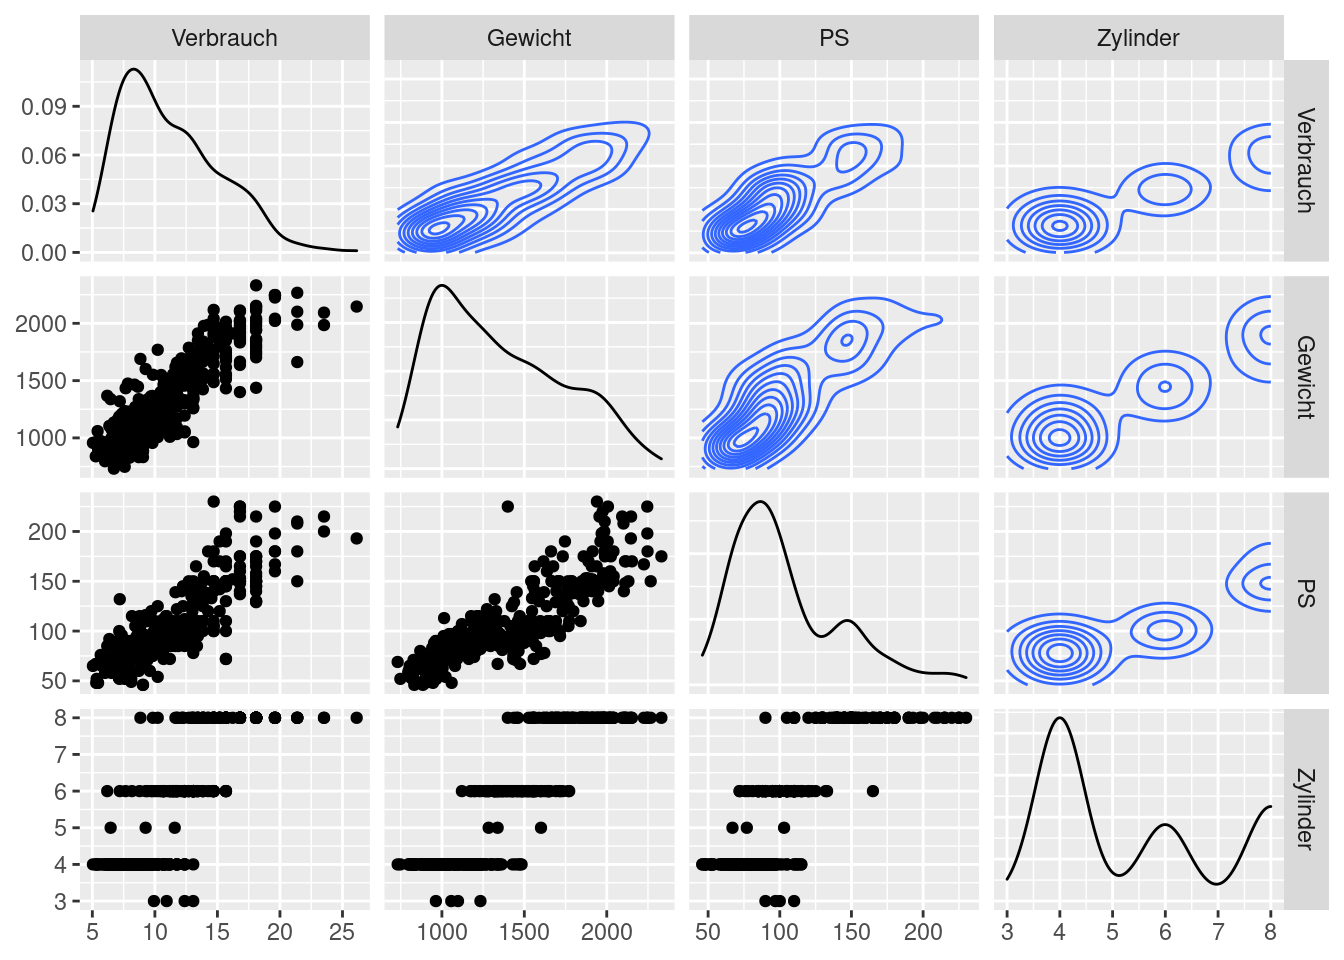
\includegraphics[width=1\linewidth]{SFDS_files/figure-latex/unnamed-chunk-11-1} \end{center}

Figure \ref{fig:GMM-plot1} zeigt das Resultat einer Clusteranalyse basierend auf einem Gaußschen Mischmodell, welches mit Hilfe des EM-Algorithmuses geschätz wurde. Das Cluster-Ergebnis ist ziemlich gut: \(95\%\) der Pinguine konnten richtig zugeordnet werden - lediglich auf Basis ihrer Flossenlängen.\\
\textbackslash begin\{figure\}{[}h{]}

\{\centering 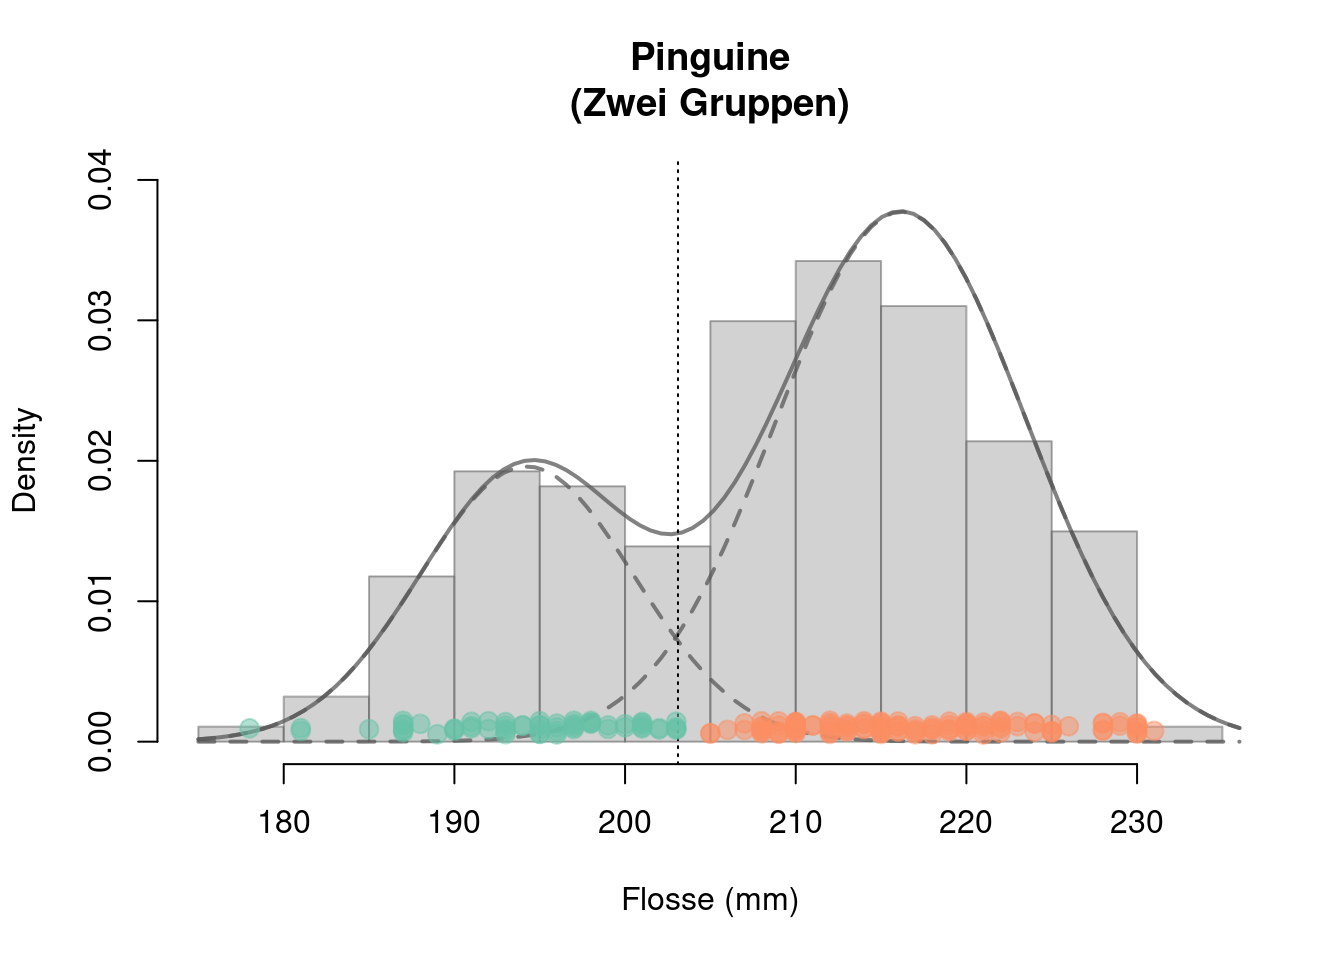
\includegraphics[width=1\linewidth]{SFDS_files/figure-latex/GMM-plot1-1}

\}

\textbackslash caption\{Zuordnung der Pinguine mit Hilfe der Bayes-Regel (hier Gruppe mit größtem Dichtewert). Auf diese Weise können 93\% der Daten korrekt zugeordnet werden.\}\label{fig:GMM-plot1}
\textbackslash end\{figure\}

\hypertarget{der-em-algorithmus-zur-ml-schuxe4tzung-gauuxdfscher-mischmodelle}{%
\section{Der EM Algorithmus zur ML-Schätzung Gaußscher Mischmodelle}\label{der-em-algorithmus-zur-ml-schuxe4tzung-gauuxdfscher-mischmodelle}}

\hypertarget{gauuxdfsche-mischmodelle-gmm}{%
\subsection{Gaußsche MischModelle (GMM)}\label{gauuxdfsche-mischmodelle-gmm}}

Eine Zufallsvariable \(X\), die einer Gauschen Mischverteilung folgt, bezeichnen wir als
\[
X\sim\mathcal{N}_{\mathcal{mix}}(G,\boldsymbol{\pi},\boldsymbol{\mu},\boldsymbol{\sigma})
\]

Die dazugehörige Dichtefunktion einer Gaußschen Mischverteilung ist folgendermaßen definiert:
\[
f_G(x|\boldsymbol{\pi},\boldsymbol{\mu},\boldsymbol{\sigma})=\sum_{g=1}^G\pi_gf(x|\mu_g\sigma_g)
\]

\begin{itemize}
\tightlist
\item
  \textbf{Gewichte:} \(\boldsymbol{\pi}=(\pi_1,\dots,\pi_G)\) mit \(\pi_g>0\) und \(\sum_{g=1}^G\pi_g=1\)
\item
  \textbf{Mittelwerte:} \(\boldsymbol{\mu}=(\mu_1,\dots,\mu_G)\) mit \(\mu_g\in\mathbb{R}\)
\item
  \textbf{Standardabweichungen:} \(\boldsymbol{\sigma}=(\sigma_1,\dots,\sigma_G)\) mit \(\sigma_g>0\)
\item
  \textbf{Normalverteilung der Gruppe \(g=1,\dots,G\):}
  \[
  f(x|\mu_g\sigma_g)=\frac{1}{\sqrt{2\pi}\sigma_g}\exp\left(-\frac{1}{2}\left(\frac{x-\mu_g}{\sigma_g}\right)^2\right)
  \]
\item
  \textbf{Unbekannte Parameter:} {\(\boldsymbol{\pi}\)}, {\(\boldsymbol{\mu}\)} und {\(\boldsymbol{\sigma}\)}
\end{itemize}

\hypertarget{maximum-likelihood-ml-schuxe4tzung}{%
\subsection{Maximum Likelihood (ML) Schätzung}\label{maximum-likelihood-ml-schuxe4tzung}}

Die unbekannten Parameter \(\boldsymbol{\pi}=(\pi_1,\dots,\pi_G)\), \(\boldsymbol{\mu}=(\mu_1,\dots,\mu_G)\) und \(\boldsymbol{\sigma}=(\sigma_1,\dots,\sigma_G)\) eines Gaußschen Mischmodells werden mit Hilfe der Maximum Likelihood Methode geschätzt.

\textbf{Wiederholung der Grundidee der ML-Schätzung:}

\begin{itemize}
\tightlist
\item
  \textbf{Annahme:} Die Daten \(\mathbf{x}=(x_1,\dots,x_n)\) sind Realisation einer einfachen (i.i.d.) Zufallsstichprobe \((X_1,\dots,X_n)\) mit
  \[ 
  X_i\sim\mathcal{N}_{\mathcal{mix}}(G,\boldsymbol{\pi},\boldsymbol{\mu},\boldsymbol{\sigma})
  \]
  und dazugehöriger Dichtefunktion \(f_G(x|\boldsymbol{\pi},\boldsymbol{\mu},\boldsymbol{\sigma})=\sum_{g=1}^G\pi_gf(x|\mu_g\sigma_g)\). D.h. die Daten \(\mathbf{x}=(x_1,\dots,x_n)\) „kennen`` die unbekannten Parameter \(\boldsymbol{\pi}\), \(\boldsymbol{\mu}\) und \(\boldsymbol{\sigma}\) und wir müssen ihnen diese Informationen „nur noch`` entlocken.
\item
  \textbf{Schätz-Idee:} Wähle \(\boldsymbol{\pi}\), \(\boldsymbol{\mu}\) und \(\boldsymbol{\sigma}\) so, dass \(f_G(\cdot|\boldsymbol{\pi},\boldsymbol{\mu},\boldsymbol{\sigma})\) \textbf{„optimal``} zu \(\mathbf{x}\) passt.
\item
  \textbf{Umsetzung:} Maximiere (bzgl. \(\boldsymbol{\pi}\), \(\boldsymbol{\mu}\) und \(\boldsymbol{\sigma}\)) die Likelihood Funktion
  \[\mathcal{L}(\boldsymbol{\pi},\boldsymbol{\mu},\boldsymbol{\sigma}|\mathbf{x})=\prod_{i=1}^nf_G(x_i|\boldsymbol{\pi},\boldsymbol{\mu},\boldsymbol{\sigma})\]
  Bzw. die Log-Likelihood Funktion (da einfacher)
  \[
  \overbrace{\ell(\boldsymbol{\pi},\boldsymbol{\mu},\boldsymbol{\sigma}|\mathbf{x})}^{=\ln\left(\mathcal{L}(\boldsymbol{\pi},\boldsymbol{\mu},\boldsymbol{\sigma}|\mathbf{x})\right)}
  =\sum_{i=1}^n\ln\left(f_G(x_i|\boldsymbol{\pi},\boldsymbol{\mu},\boldsymbol{\sigma})\right)
  =\sum_{i=1}^n\ln\left(\sum_{g=1}^G\pi_g\phi_{\mu_g\sigma_g}(x_i)\right)
  \]
\item
  Die \(\ell\) maximierenden Parameterwerte {\(\hat{\boldsymbol{\pi}}\)}, {\(\hat{\boldsymbol{\mu}}\)} und {\(\hat{\boldsymbol{\sigma}}\)} sind die {\textbf{ML-Schätzer}}. Das kann man so ausdrücken:
  \[
  (\hat{\boldsymbol{\pi}},\hat{\boldsymbol{\mu}},\hat{\boldsymbol{\sigma}}=\arg\min_{(\boldsymbol{\pi},\boldsymbol{\mu},\boldsymbol{\sigma})}\ell(\boldsymbol{\pi},\boldsymbol{\mu},\boldsymbol{\sigma}|\mathbf{x})
  \]
\end{itemize}

\hypertarget{die-ml-schuxe4tzer-hatboldsymbolpi-hatboldsymbolmu-und-hatboldsymbolsigma}{%
\subsection*{\texorpdfstring{Die ML-Schätzer \(\hat{\boldsymbol{\pi}}\), \(\hat{\boldsymbol{\mu}}\) und \(\hat{\boldsymbol{\sigma}}\)}{Die ML-Schätzer \textbackslash hat\{\textbackslash boldsymbol\{\textbackslash pi\}\}, \textbackslash hat\{\textbackslash boldsymbol\{\textbackslash mu\}\} und \textbackslash hat\{\textbackslash boldsymbol\{\textbackslash sigma\}\}}}\label{die-ml-schuxe4tzer-hatboldsymbolpi-hatboldsymbolmu-und-hatboldsymbolsigma}}
\addcontentsline{toc}{subsection}{Die ML-Schätzer \(\hat{\boldsymbol{\pi}}\), \(\hat{\boldsymbol{\mu}}\) und \(\hat{\boldsymbol{\sigma}}\)}

Analytische Lösungen (Herleitungen sind lästig aber machbar - siehe Übungsaufgaben):
\[
\begin{align*}
\hat\pi_g&=\frac{1}{n}\sum_{i=1}^np_{ig}\\
\hat\mu_g&=\sum_{i=1}^n\frac{p_{ig}}{\left(\sum_{j=1}^np_{jg}\right)}x_i\\
\hat\sigma_g&=\sqrt{\sum_{i=1}^n\frac{p_{ig}}{\left(\sum_{j=1}^np_{jg}\right)}\left(x_i-\hat\mu_g\right)^2},\quad g=1,\dots,G
\end{align*}
\]

🙈 {\textbf{Aber:}}
\[
% p_{ig}=\frac{\pi_g\phi_{\mu_g\sigma_g}(x_i)}{\sum_{l=1}^G\pi_l\phi_{\mu_l\sigma_l}(x_i)},\quad i=1,\dots,n;\;g=1,\dots,G
p_{ig}=\frac{\pi_g\phi_{\mu_g\sigma_g}(x_i)}{f_G(x_i|\boldsymbol{\pi},\boldsymbol{\mu},\boldsymbol{\sigma})}
\]
hängt, für alle \(i=1,\dots,n\) und \(g=1,\dots,G\), von den {\textbf{unbekannten}} Parametern \(\boldsymbol{\pi}\), \(\boldsymbol{\mu}\) und \(\boldsymbol{\sigma}\) ab.

🥳 {\textbf{Lösung: Der EM Algorithmus}}

\hypertarget{der-em-algorithmus-fuxfcr-gauuxdfsche-mischmodelle}{%
\section{Der EM Algorithmus für Gaußsche Mischmodelle}\label{der-em-algorithmus-fuxfcr-gauuxdfsche-mischmodelle}}

Die Idee des EM Algorithmus ist einfach und folgt einem iterativen Schema: Starte mit errateten Werten für \(\boldsymbol{\pi}^{(0)}\), \(\boldsymbol{\mu}^{(0)}\) und \(\boldsymbol{\sigma}^{(0)}\). In der \(k\)ten Wiederholung (\(k=1,2,\dots\)) kann man, erstens, neue \(p_{ig}^{(r)}\) Werte berechnen (basierend auf \(\boldsymbol{\pi}^{(r-1)}\), \(\boldsymbol{\mu}^{(r-1)}\) und \(\boldsymbol{\sigma}^{(r-1)}\)) und, zweitens, neue ML-Schätzer \(\boldsymbol{\pi}^{(r)}\), \(\boldsymbol{\mu}^{(r)}\) und \(\boldsymbol{\sigma}^{(r)}\) berechnen (basierend auf den neuen \(p_{ig}^{(r)}\)). Dies wiederholt man bis die Schätzung konvergiert (sich nicht mehr ändert).

\textbf{Der Der EM Algorithmus:}

\begin{enumerate}
\def\labelenumi{\arabic{enumi}.}
\item
  Setze Startwerte \(\boldsymbol{\pi}^{(0)}\), \(\boldsymbol{\mu}^{(0)}\) und \(\boldsymbol{\sigma}^{(0)}\)
\item
  Für \(r=1,2,\dots\)

  \begin{itemize}
  \item
    {\textbf{(Expectation)}} Berechne:
    \[p_{ig}^{(r)}=\frac{\pi_g^{(r-1)}\phi_{\mu^{(r-1)}_g\sigma_g^{(r-1)}}(x_i)}{f_G(x_i|\boldsymbol{\pi}^{(r-1)},\boldsymbol{\mu}^{(r-1)},\boldsymbol{\sigma}^{(r-1)})}\]
  \item
    {\textbf{(Maximization)}} Berechne:

    \(\hat\pi_g^{(r)}=\frac{1}{n}\sum_{i=1}^np_{ig}^{(r)},\quad\quad\hat\mu_g^{(r)}=\sum_{i=1}^n\frac{p_{ig}^{(r)}}{\left(\sum_{j=1}^np_{jg}^{(r)}\right)}x_i\)

    \(\hat\sigma_g^{(r)}=\sqrt{\sum_{i=1}^n\left(p_{ig}^{(r)}\Big/\sum_{j=1}^np_{jg}^{(r)}\right)\left(x_i-\hat\mu_g^{(r)}\right)^2}\)
  \end{itemize}
\item
  Prüfe Konvergenz
\end{enumerate}

\begin{Shaded}
\begin{Highlighting}[]
\KeywordTok{library}\NormalTok{(}\StringTok{"MASS"}\NormalTok{)}
\KeywordTok{library}\NormalTok{(}\StringTok{"mclust"}\NormalTok{)}

\CommentTok{## Daten:}
\NormalTok{x <-}\StringTok{ }\KeywordTok{cbind}\NormalTok{(Penguine_Flosse) }\CommentTok{# Daten [n x d]-Dimensional. }
\NormalTok{d <-}\StringTok{ }\KeywordTok{ncol}\NormalTok{(x)                }\CommentTok{# Dimension (d=1: univariat)}
\NormalTok{n <-}\StringTok{ }\KeywordTok{nrow}\NormalTok{(x)                }\CommentTok{# Stichprobenumfang}
\NormalTok{G <-}\StringTok{ }\DecValTok{2}                      \CommentTok{# Anzahl Gruppen}


\CommentTok{## 1. Startwerte für pi, mu und sigma:}
\NormalTok{tau   <-}\StringTok{ }\KeywordTok{rep}\NormalTok{(}\DecValTok{1}\OperatorTok{/}\NormalTok{G, G)              }\CommentTok{# Naive pi}
\NormalTok{sigma <-}\StringTok{ }\KeywordTok{array}\NormalTok{(}\KeywordTok{diag}\NormalTok{(d), }\KeywordTok{c}\NormalTok{(d,d,G)) }\CommentTok{# Varianz = 1}
\NormalTok{mu    <-}\StringTok{ }\KeywordTok{t}\NormalTok{(MASS}\OperatorTok{::}\KeywordTok{mvrnorm}\NormalTok{(G, }\KeywordTok{colMeans}\NormalTok{(x), sigma[,,}\DecValTok{1}\NormalTok{]}\OperatorTok{*}\DecValTok{4}\NormalTok{) )}

\CommentTok{## Weitere Deklarationen:}
\NormalTok{llk       <-}\StringTok{ }\KeywordTok{matrix}\NormalTok{(}\OtherTok{NA}\NormalTok{, n, G)}
\NormalTok{p         <-}\StringTok{ }\KeywordTok{matrix}\NormalTok{(}\OtherTok{NA}\NormalTok{, n, G)  }
\NormalTok{loglikOld <-}\StringTok{ }\FloatTok{1e07}
\NormalTok{tol       <-}\StringTok{ }\FloatTok{1e-05}
\NormalTok{it        <-}\StringTok{ }\DecValTok{0}
\NormalTok{check     <-}\StringTok{ }\OtherTok{TRUE} 


\CommentTok{## EM Algorithmus}
\ControlFlowTok{while}\NormalTok{(check)\{}
  
  \CommentTok{## Expectation-Schritt }
  \ControlFlowTok{for}\NormalTok{(g }\ControlFlowTok{in} \DecValTok{1}\OperatorTok{:}\NormalTok{G)\{}
\NormalTok{    p[,g] <-}\StringTok{ }\NormalTok{tau[g] }\OperatorTok{*}\StringTok{ }\NormalTok{mclust}\OperatorTok{:::}\KeywordTok{dmvnorm}\NormalTok{(x, mu[,g], sigma[,,g])}
\NormalTok{  \}}
\NormalTok{  p <-}\StringTok{ }\KeywordTok{sweep}\NormalTok{(p, }\DecValTok{1}\NormalTok{, }\DataTypeTok{STATS =} \KeywordTok{rowSums}\NormalTok{(p), }\DataTypeTok{FUN =} \StringTok{"/"}\NormalTok{)}
  
  \CommentTok{# Maximization-Schritt:}
\NormalTok{  par   <-}\StringTok{ }\NormalTok{mclust}\OperatorTok{::}\KeywordTok{covw}\NormalTok{(x, p, }\DataTypeTok{normalize =} \OtherTok{FALSE}\NormalTok{)}
\NormalTok{  mu    <-}\StringTok{ }\NormalTok{par}\OperatorTok{$}\NormalTok{mean}
\NormalTok{  sigma <-}\StringTok{ }\NormalTok{par}\OperatorTok{$}\NormalTok{S}
\NormalTok{  tau   <-}\StringTok{ }\KeywordTok{colMeans}\NormalTok{(p)}
  
  \CommentTok{## Berechnung des aktuellen Wertes der Log-Likelihood Funktion}
  \ControlFlowTok{for}\NormalTok{(g }\ControlFlowTok{in} \DecValTok{1}\OperatorTok{:}\NormalTok{G) \{}
\NormalTok{    llk[,g] <-}\StringTok{ }\NormalTok{tau[g] }\OperatorTok{*}\StringTok{ }\NormalTok{mclust}\OperatorTok{:::}\KeywordTok{dmvnorm}\NormalTok{(x, mu[,g], sigma[,,g])}
\NormalTok{  \}}
\NormalTok{  loglik <-}\StringTok{ }\KeywordTok{sum}\NormalTok{(}\KeywordTok{log}\NormalTok{(}\KeywordTok{rowSums}\NormalTok{(llk)))}
  
  \CommentTok{## Prüfung der Konvergenz}
\NormalTok{  diff      <-}\StringTok{ }\KeywordTok{abs}\NormalTok{(loglik }\OperatorTok{-}\StringTok{ }\NormalTok{loglikOld)}\OperatorTok{/}\KeywordTok{abs}\NormalTok{(loglik)}
\NormalTok{  loglikOld <-}\StringTok{ }\NormalTok{loglik}
\NormalTok{  it        <-}\StringTok{ }\NormalTok{it }\OperatorTok{+}\StringTok{ }\DecValTok{1}
\NormalTok{  check     <-}\StringTok{ }\NormalTok{diff }\OperatorTok{>}\StringTok{ }\NormalTok{tol}
\NormalTok{\}}
\end{Highlighting}
\end{Shaded}

\hypertarget{vervollstuxe4ndigung-der-daten-durch-latente-variablen-der-wahre-blick-auf-den-em-algorithmus}{%
\section{Vervollständigung der Daten durch Latente Variablen: Der wahre Blick auf den EM-Algorithmus}\label{vervollstuxe4ndigung-der-daten-durch-latente-variablen-der-wahre-blick-auf-den-em-algorithmus}}

Pinguin-Daten: Es gibt zwei Gruppen (\(g\in\{1,2\}\)). Ist gäbe im Prinzip also eine „latente`` (d.h. unbeobachtete) Zuordnung \(z_{ig}\):
\[
z_{ig}=
\left\{\begin{array}{ll}
1&\text{falls Pinguin }i\text{ zu Gruppe }g\text{ gehört.}\\
0&\text{sonst.}\\
\end{array}\right.,
\]
wobei es für jeden Pinguin \(i\) nur \textbf{eine} Gruppe gibt (falls \(z_{i1}=1\) dann \(z_{i2}=0\)). Dies ist eine wichtige Restriktion (jede Beobachtung nur eine Gruppe), welche bei den Pinguinen unproblematisch ist, in anderen Kontexten jedoch problematisch sein kann.

Die Zuordnungsvariablen \(\mathbf{z}=(z_{11},\dots,z_{nG})\) sind leider unbekannt (latent). Wir wissen aber trotzdem etwas über diese Zuordnungen. Laut unserem Modell
\[
f_G(x|\boldsymbol{\pi},\boldsymbol{\mu},\boldsymbol{\sigma})=\sum_{g=1}^G\pi_gf(x|\mu_g\sigma_g),
\]
ist die Zuordnung \(z_{ig}\) nämlich eine Realisation einer Bernoulli Zufallsvariable
\[
Z_{ig}\sim\mathcal{B}(\pi_g)
\]
Also
\[
\begin{align*}
P(Z_{ig}=1)&=\;\;\;\pi_g\;\;=P(\text{Pinguin $i$ gehört zu Gruppe }g)\\
P(Z_{ig}=0)&=1-\pi_g=P(\text{Pinguin $i$ gehört nicht zu Gruppe }g)
\end{align*}
\]
Man nennt \(\pi_1,\dots,\pi_G\) hier die \textbf{„a-priori-Wahrscheinlichkeiten``}. Wenn wir nichts über die Flossenlänge von Pinguin \(i\) wissen, dann bleiben uns nur die a-priori-Wahrscheinlichkeiten: Mit Wahrscheinlichkeit \(\pi_g\) gehört Pinguin \(i\) zu Gruppe \(g\).

\textbf{A-posteriori-Wahrscheinlichkeit \(\;p_{ig}\):}

(Satz von Bayes)
\[
\begin{align*}
p_{ig}
&=\frac{\pi_g\phi_{\mu_g\sigma_g}(x_i)}{f_G(x_i|\boldsymbol{\pi},\boldsymbol{\mu},\boldsymbol{\sigma})}\\[2ex]
&=\frac{\overbrace{P(Z_{ig}=1)}^{\text{„A-priori-Wahrs.“}}\phi_{\mu_g\sigma_g}(x_i)}{f_G(x_i|\boldsymbol{\pi},\boldsymbol{\mu},\boldsymbol{\sigma})}=\overbrace{P(Z_{ig}=1|X_i=x_i)}^{\text{„A-posteriori-Wahrs.“}}=p_{ig}\\
\end{align*}
\]
Beachte: \(p_{ig}\) ist ein (bedingter) Mittelwert {\textbf{(Expectation)}}
\[
\begin{align*}
p_{ig}&=\underbrace{1\cdot P(Z_{ig}=1|X_i=x_i)+0\cdot P(Z_{ig}=0|X_i=x_i)}_{=E(Z_{ig}=1|X_i=x_i)}\\
\end{align*}
\]

\hypertarget{der-em-algorithmus}{%
\subsection*{\texorpdfstring{Der {E}{M} Algorithmus}{Der EM Algorithmus}}\label{der-em-algorithmus}}
\addcontentsline{toc}{subsection}{Der {E}{M} Algorithmus}

\begin{enumerate}
\def\labelenumi{\arabic{enumi}.}
\item
  Setze Startwerte \(\boldsymbol{\pi}^{(0)}\), \(\boldsymbol{\mu}^{(0)}\) und \(\boldsymbol{\sigma}^{(0)}\)
\item
  Für \(r=1,2,\dots\)

  \begin{itemize}
  \item
    {\textbf{(Expectation)} } Berechne:\\

    \(p_{ig}^{(r)}=E\left(Z_{ig}^{(r-1)}\left|X_i^{(r-1)}=x_i\right.\right)\)

    \(\begin{align*}  \text{wobei }\;Z_{ig}^{(r-1)}&\sim\mathcal{B}\left(\pi_g^{(r-1)}\right)\\  \text{und }\;X_i^{(r-1)}&\sim \mathcal{N}_{\mathcal{mix}}(G,\boldsymbol{\pi}^{(r-1)},\boldsymbol{\mu}^{(r-1)},\boldsymbol{\sigma}^{(r-1)})  \end{align*}\)
  \item
    {\textbf{(Maximization)}} Berechne: \(\hat\pi_g^{(r)}\), \(\hat\mu_g^{(r)}\), \(\hat\sigma_g^{(r)}\)
  \end{itemize}
\item
  Prüfe Konvergenz
\end{enumerate}

--\textgreater{}

  \bibliography{book.bib,packages.bib}

\end{document}
